% This file is part of Cities and Libraries: A Connected Component Problem.
% Copyright (C) 2024 Nicholas Fleischhauer
%
% Cities and Libraries: A Connected Component Problem is free software: you can redistribute it and/or modify
% it under the terms of the GNU General Public License as published by
% the Free Software Foundation, either version 3 of the License, or
% (at your option) any later version.
%
% Cities and Libraries: A Connected Component Problem is distributed in the hope that it will be useful,
% but WITHOUT ANY WARRANTY; without even the implied warranty of
% MERCHANTABILITY or FITNESS FOR A PARTICULAR PURPOSE. See the
% GNU General Public License for more details.
%
% You should have received a copy of the GNU General Public License
% along with Cities and Libraries: A Connected Component Problem. If not, see <https://www.gnu.org/licenses/>.

\documentclass[11pt, a4paper, oneside]{article}

\title{Cities and Libraries: A Connected Component Problem}
\author{Nicholas Fleischhauer}
\date{\today}

% Encoding and language support
\usepackage[utf8]{inputenc}
\usepackage[english]{babel}
% \usepackage{csquotes}

% Mathematical packages
\usepackage{amsmath, amssymb, amsthm}

% Graphics, tables, and layout
\usepackage{graphicx}
\usepackage{float}
\usepackage[inner=1.5cm, outer=1.5cm, top=2.5cm, bottom=2.5cm]{geometry}
\graphicspath{{assets/}}

% Algorithms
\usepackage{algorithm, algpseudocode}

% Colors and fancy text
\usepackage[usenames, dvipsnames, svgnames, table]{xcolor}
\usepackage{fancyhdr}

\setlength{\headheight}{13.6pt}

% Custom colors
\definecolor{darkblue}{rgb}{0,0,.6}
\definecolor{darkred}{rgb}{.7,0,0}
\definecolor{darkgreen}{rgb}{0,.6,0}
\definecolor{red}{rgb}{.98,0,0}
\definecolor{OliveGreen}{cmyk}{0.64,0,0.95,0.40}
\definecolor{CadetBlue}{cmyk}{0.62,0.57,0.23,0}
\definecolor{lightlightgray}{gray}{0.93}

% Bibliography management
\usepackage[backend=biber, style=authoryear, citestyle=authoryear]{biblatex}
\addbibresource{references.bib}

% Page footer management
\usepackage{lastpage}

% For code blocks
\usepackage{minted}

\usepackage{csquotes}

% For paragraph formatting
\usepackage{parskip}
\setlength{\parskip}{10pt plus 1pt minus 1pt}

% Hyperlinks
\usepackage{hyperref}
\hypersetup{
    pdfauthor={Nicholas Fleischhauer},
    pdftitle={Cities and Libraries: A Connected Component Problem},
    pdfsubject={GNU General Public License},
    pdfkeywords={GPL, License, LaTeX, Connected Components},
    pdfproducer={GNU General Public License v3.0 or later, see https://www.gnu.org/licenses/gpl-3.0.en.html},
    colorlinks=true,
    linkcolor=darkred,
    filecolor=magenta,
    urlcolor=darkblue,
    citecolor=darkblue,
    bookmarksnumbered=true,
    plainpages=false
}

% Verbatim and special text environments
\usepackage{verbatim, fancyvrb}
\VerbatimFootnotes

% Page header and footer style
\pagestyle{fancy}
\fancyhf{}
\lhead{Cities and Libraries: A Connected Component Problem}
\rhead{\date{\today}}
% \fancyfoot[C]{Page \thepage\ of \pageref*{LastPage}}
\fancyfoot[C]{\scriptsize Page \thepage\ of \pageref*{LastPage} \textbar{} Licensed under the GNU GPL v3.0 or later}

% Custom mathematical commands
\newcommand{\R}{\mathbb{R}}
\newcommand{\F}{\mathbb{F}}
\newcommand{\LL}{\mathcal{L}}
\newcommand{\C}{\mathbb{C}}
\newcommand{\spn}{\operatorname{span}}
\newcommand{\nll}{\operatorname{null}}
\newcommand{\range}{\operatorname{range}}

% Theorems
\newtheorem{theorem}{Theorem}
\newtheorem{proposition}{Proposition}

\begin{document}

\maketitle

\begin{abstract}
  This paper analyzes an algorithmic problem involving the optimization of library and road construction in a network of cities. By refining the problem statement and exploring connected components within graphs, we develop a cost-minimizing strategy and implement an efficient solution. Custom visualizations and detailed explanations support the methodology and findings presented.
\end{abstract}
  

\section*{Introduction}

In the realm of interview preparation, solving algorithmic problems is a common practice to assess and enhance one's problem-solving skills. This paper presents an analysis of a specific problem sourced from HackerRank \cite{hackerrank}, focusing on optimizing the allocation of libraries and roads within a network of cities.

\begin{itemize}
  \item \textbf{Problem Refinement:} We begin by presenting a refined version of the original problem, addressing and correcting various errors and informational inconsistencies that often accompany such "toy" problems.
  \item \textbf{Thought Process and Optimization:} Following the problem statement, we detail the thought process involved in approaching and solving the problem optimally, highlighting key strategies and considerations.
  \item \textbf{Coded Solution:} Finally, we provide a comprehensive coded solution, illustrating the implementation of the discussed methodologies.
\end{itemize}

To facilitate a clear understanding of the concepts discussed, custom visualizations of graphs and connected components were generated using the Manim mathematical animation framework \cite{manim}.


\section*{Problem Statement}

As a city planner, your task is to provide the citizens of HackerLand with access to libraries while minimizing the overall infrastructure costs.

\subsection*{Task}

Determine the minimum cost to provide library access to all citizens of HackerLand.

\subsection*{Initial Setup}
There are \(n\) cities numbered from \(1\) to \(n\). Currently there are no libraries and the cities are not connected. Bidirectional roads may be built between any city pair listed in \textit{city\_edges}.

A citizen has access to a library if:

\begin{itemize}
  \item Their city contains a library or ...
  \item They can travel by road from their city to another city containing a library.
\end{itemize}

For example, if a citizen of city \(1\) doesn't have a library, but city \(2\) has a library and both cities are connected by a road, then all citizens of city \(1\) have access to a library and all citizens of city \(2\) have acces to a library.

\subsection*{Example Problem}

The following figure is a sample map of HackerLand, where the dotted lines denote possible roads:

\begin{figure}[H]
  \centering
  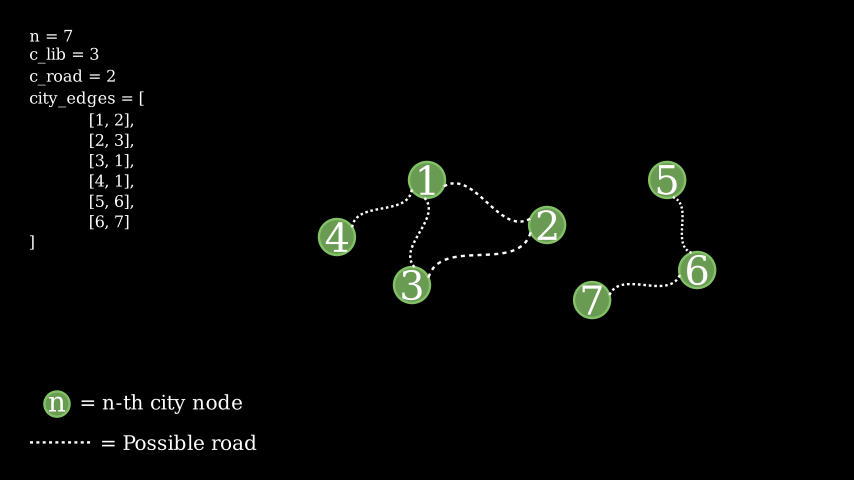
\includegraphics[width=0.5\textwidth]{hackerland-graph.png}
  \caption{Map of HackerLand illustrating possible road connections}
  \label{fig:image1}
\end{figure}

The inputs for this example are as follows:

\begin{itemize}
  \item \(n = 7\), the number of cities
  \item \(c_{\text{lib}} = 3\), the cost of a single library
  \item \(c_{\text{road}} = 2\), the cost of a single road
  \item \(city\_edges = [[1, 2], [2, 3], [3, 1], [4, 1], [5, 6], [6, 7]]\), a list of \textit{pontential} connections between cities i.e, where a road can be built but hasn't been built yet. (Assume we can't build a road between node \(2\) and \(7\) for example)
\end{itemize}

\subsection*{Example Solution}

The minimal cost solution for this example is to build \(5\) roads and \(2\) libraries. So the total cost of this is

\[\text{Total Cost} = (5) \times 2 + (2) \times 3 = 16\]

note that\textit{ one of the possible roads in the cycle} \(1 \rightarrow 2 \rightarrow 3\) \textit{is unnecessary}.

% \clearpage
\section*{Coding Setup}

\subsection*{Function Description}

Complete the function \textbf{roads\_and\_libraries}

\begin{minted}[linenos, frame=lines]{python}
from typing import List

def roads_and_libraries(n: int, c_lib: int, c_road: int, city_edges: List[List[int]]) -> int:
  """
    Determines the minimum cost to provide library access to all citizens of HackerLand.

    Args:
        n (int): The number of cities.
        c_lib (int): The cost to build a single library.
        c_road (int): The cost to build a single road.
        city_edges (List[List[int]]): A list of edges representing possible roads between cities.
            Each sublist contains two integers indicating a bidirectional road
            between the specified cities.

    Returns:
        int: The minimal total cost to ensure all citizens have access to a library.

    Example:
        >>> n = 7
        >>> c_lib = 3
        >>> c_road = 2
        >>> city_edges = [[1, 2], [2, 3], [3, 1], [4, 1], [5, 6], [6, 7]]
        >>> roads_and_libraries(n, c_lib, c_road, city_edges)
        16
    """
  ...
\end{minted}

\subsection*{Command Line Input Format}

The following is the command line input format for testing purposes.

\begin{minted}[linenos, frame=lines]{text}
  q
  n m c_lib c_road
  u_i v_i
\end{minted}

where:

\begin{itemize}
  \item \(q\) is the number of queries
  \item \(m\) is the number of potential roads contained within \(city_{edges}\)
  \item \(c_{\text{lib}}\) is the cost to build a library
  \item \(c_{\text{road}}\) is the cost to build a road
  \item \(u_{i}\) and \(v_{i}\) are the \(i\)-th pair of cities that can be connected by a potential road
\end{itemize}

\subsection*{Input Constraints}

\begin{itemize}
  \item \(1 \leq q \leq 10\)
  \item \(1 \leq n \leq 10^{5}\)
  \item \(0 \leq m \leq min \left(10^{5}, \frac{n\cdot(n - 1)}{2} \right)\)
  \item \(1 \leq c_{lib}, c_{\text{road}} \leq 10^{5}\)
  \item \(1 \leq u_{i}, v_{i} \leq n\)
  \item each potential road connects two distinct cities
\end{itemize}

\subsection*{Command Line Input Format Example}

An example is provided with two queries. The first query matches the example problem shown in Figure~\ref{fig:image1}, representing the layout of HackerLand, and the second query pertains to another land, Scriptshire, as shown in Figure~\ref{fig:image2}.

\begin{figure}[H]
  \centering
  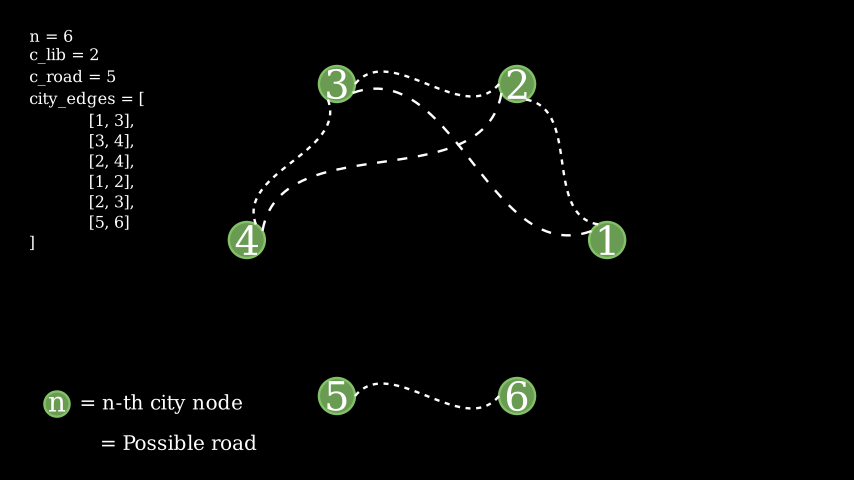
\includegraphics[width=0.5\textwidth]{scriptshire-graph.png}
  \caption{Scriptshire}
  \label{fig:image2}
\end{figure}

\subsection*{Command Line Input Format Example}

\begin{minted}[linenos, frame=lines]{text}
  STDIN       Function
  -----       --------
  2           q = 2
  7 6 3 2     n = 7, city_edges[] size m = 6, c_lib = 3, c_road = 2
  1 2         city_edges = [[1, 2], [2, 3], [3, 1], [4, 1], [5, 6], [6, 7]]
  2 3
  3 1
  4 1
  5 6
  6 7
  6 6 2 5     n = 6, city_edges[] size m = 6, c_lib = 2, c_road = 5
  1 3         city_edges = [[1, 3], [3, 4],...]
  3 4
  2 4
  1 2
  2 3
  5 6
\end{minted}

\subsection*{Sample Output}

The following is the sample output for the inputs used above.

\begin{minted}[linenos, frame=lines]{text}
  16
  12
\end{minted}

\subsection*{Explanation}

The cheapest way to make libraries accessible to all \textbf{for HackerLand} is to:

\begin{itemize}
  \item Build a single library within any of the cities in the first component at a cost of \(3\).
  \item Build roads between each city within the first component such that each city can reach one another either directly, or via another city by road.
  \item The same holds for the second component.
\end{itemize}

This results in a total cost of \((3 \times 2 + 1 \times 3) + (2 \times 2 + 1 \times 3) = 16\), where the first component requires:

\begin{itemize}
  \item \(3\) roads at a cost of \(2\) each
  \item \(1\) library at the cost of \(3\) each
\end{itemize} 

and the second component requires:

\begin{itemize}
  \item \(2\) roads at a cost of \(2\) each
  \item \(1\) library at a cost of \(3\) each
\end{itemize}

The most economical way to provide library access to all in \textbf{Scriptshire} is to build a library in each city because the cost to build a library (2) is less than the cost to build a road (5). Scriptshire contains 6 cities, so the minimal total cost is \(6 \times 2 = 12\).

\section*{Diving Into the Problem}

Our objective is to ensure that all citizens have access to a library while minimizing the overall cost. To achieve this, we need to define an appropriate cost function. Before formulating the cost function, we present some preliminary observations.

\subsection*{Observations and Thoughts}

\begin{enumerate}
  \item A well-known mathematical formula related to triangular numbers \cite{triangularnumber} appears in the constraint bounds:
    \[
    0 \leq m \leq \min \left(10^{5}, \frac{n(n - 1)}{2}\right)
    \]
  \item Connecting each city to all other cities would result in \(\frac{n(n - 1)}{2}\) roads, which is often more than necessary. For example, in HackerLand (Figure~\ref{fig:image1}), seven nodes would require 21 roads for full connectivity, but our optimal solution uses only five roads.
  \item The cost function is inherently tied to the concept of connected components.
  \item In the case of HackerLand, there are two connected components. Each component requires at least one library.
  \item Therefore, the lower bound on the number of libraries is one per connected component.
  \item For each connected component, there are two possible strategies:
    \begin{itemize}
      \item Build one library and construct roads to connect all cities within the component.
      \item Build libraries in all cities within the component.
    \end{itemize}
\end{enumerate}

\subsection*{Clarification on Connected Components}

A connected component \cite{graphcomponent} is a subset of a larger structure (e.g., HackerLand) where every pair of elements within the subset is connected by some defined relationship. In our case, these are the dashed lines indicating where a potential road can be built.

\begin{figure}[H]
  \centering
  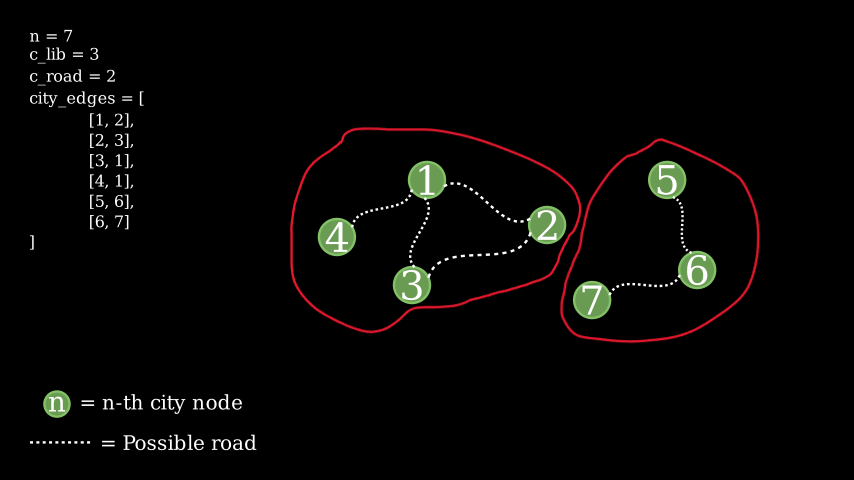
\includegraphics[width=0.5\textwidth]{connected-component-example.png}
  \caption{two connected components}
  \label{fig:image3}
\end{figure}


\subsection*{Defining the Cost Function}

Next, we explore how to define our cost function, starting at the component level.

\subsection*{Game Plan}

\begin{enumerate}
  \item Define a mathematical function that represents cost at the \textbf{component level}.
  \item Identify edge cases.
  \item Determine when minimal cost is achieved, at the \textbf{component level}, in terms of options that account for the edge cases and pickrove that minimal \textbf{component cost} is achieved. 
  \item Define a mathematical function that represents the \textbf{total cost} in terms of components.
  \item Show that \textbf{total cost} is minimized as a consequence of all \textbf{component costs} being minimized. 
\end{enumerate}

\subsubsection*{Component Cost Function}

Within each connected component, we can treat the number of cities \( k \) as a fixed constant since it remains unchanged. Our focus is on how many libraries \( s \) are needed within it.

Let:

\begin{itemize}
  \item \(k\) be the number of cities.
  \item \(s\) be the number of libraries.
  \item \(r\) be the number of roads.
\end{itemize}

where \( 1 \leq s \leq k \) and \( 0 \leq r \leq k - 1 \).

Our options can then be broken down into the following table:

\begin{table}[H]
  \centering
  \begin{tabular}{|c|c|}
    \hline
    \textbf{Libraries (\( s \))} & \textbf{Roads (\( r \))} \\ \hline
    \rowcolor{green!15} 1 & \( k - 1 \) \\ \hline
    2 & \( k - 2 \) \\ \hline
    \vdots & \vdots \\ \hline
    \( k - 1 \) & 1 \\ \hline
    \rowcolor{green!15} \( k \) & 0 \\ \hline
  \end{tabular}
  \caption{Relationship between the Number of Libraries (\( s \)) and Roads (\( r \)) in a Connected Component}
  \label{tab:libraries-roads}
\end{table}

The table reveals a pattern that shows a linear relationship between the number of libraries and roads:

\[s + r = k\]

For each additional library built, one fewer road is needed to connect the remaining cities.

We can now define the cost function as:

\[
C(s) = s \times c_{\text{lib}} + r \times c_{\text{road}}
\]

Since \( r = k - s \), we can express the cost function entirely in terms of \( s \) and \( k \). Thus, for each connected component with \( k \) cities, the cost is:

\[
C(s) = s \times c_{\text{lib}} + (k - s) \times c_{\text{road}}
\]

\subsubsection*{Edge Cases}

\begin{itemize}
  \item \(c_{\text{lib}} \leq c_{\text{road}}\): Building libraries in all cities is always cheaper or equal in cost to building roads. The code should naturally handle this case because the cost of libraries in all cities will be less than or equal to a single library with all roads.
  \item When \(c_{\text{road}}\) is very high: The cost of building roads might make the cost of one library with roads higher than the cost of libraries in all cities. The code should correctly choose to build libraries in all cities in this scenario.
\end{itemize}

\subsubsection*{Minimal Cost at the Component Level}

To ensure minimal cost, we need to consider the options for each connected component and choose the cheaper one.

\begin{theorem}
For a connected component with \( k \) cities, the minimal cost is given by:
\[
\min (C(s)) = \min \left( k \times c_{\text{lib}},\ c_{\text{lib}} + (k - 1) \times c_{\text{road}} \right)
\]
where \( C(s) \) is the total cost, \( c_{\text{lib}} \) is the cost of building a library, and \( c_{\text{road}} \) is the cost of building a road.
\end{theorem}

\begin{proof}
We analyze the cost function:
\[
C(s) = s \times c_{\text{lib}} + (k - s) \times c_{\text{road}}
\]
where \( s \) is the number of libraries, \( r = k - s \) is the number of roads, and \( 1 \leq s \leq k \).

\textbf{Case 1:} \( c_{\text{lib}} > c_{\text{road}} \)

- \( c_{\text{lib}} - c_{\text{road}} > 0 \)
- The cost function \( C(s) \) increases as \( s \) increases.
- \textbf{Minimum Total Cost}: Achieved when \( s = 1 \) (one library and \( k - 1 \) roads).

\textbf{Case 2:} \( c_{\text{lib}} < c_{\text{road}} \)

- \( c_{\text{lib}} - c_{\text{road}} < 0 \)
- The cost function \( C(s) \) decreases as \( s \) increases.
- \textbf{Minimum Total Cost}: Achieved when \( s = k \) (libraries in all cities and no roads).

\textbf{Case 3:} \( c_{\text{lib}} = c_{\text{road}} \)

- \( c_{\text{lib}} - c_{\text{road}} = 0 \)
- The cost function \( C(s) \) is constant with respect to \( s \).
- Any number of libraries between \( 1 \) and \( k \) yields the same total cost.

In each case, intermediate values of \( s \) do not provide a lower cost than the endpoints \( s = 1 \) or \( s = k \). Therefore, the minimal cost is achieved by choosing the option that results in the lower cost between building one library with roads or building libraries in all cities.
\end{proof}

Based on this analysis, our optimal strategy simplifies to:

\begin{itemize}
  \item \textbf{If} \( c_{\text{lib}} \geq c_{\text{road}} \): Build one library and construct roads to connect all cities within the component.
  \item \textbf{If} \( c_{\text{lib}} \leq c_{\text{road}} \): Build a library in each city within the component.
\end{itemize}

\subsubsection*{Total Cost Function}

The total cost of the infrastructure project can be represented as the sum of the cost of each component.

\[\text{Total Cost} = \sum_{\text{all components}} C(s)\]

Since we've minimized the costs on a per component basis, the total cost is also minimized.

\section*{Algorithm Solution Overview}

The algorithm employs a Breadth-First Search (BFS) to identify connected components within the graph representing the cities and potential roads. For each connected component, we calculate the minimal cost based on the previously defined cost function, choosing between building libraries in all cities or building one library and connecting the remaining cities with roads.

\subsection*{Implementation Code}

We have all the pieces solved, now its just a matter of implementing them in code.

\subsubsection*{Game Plan}

\begin{enumerate}
  \item Create a method for identifying connected components.
  \item For each component, apply the minimal cost function.
  \item Aggregate all the minimum costs to get the total minimum cost.
\end{enumerate}

To achieve this, we build a graph from the adjacency list (\( \text{city\_edges} \)) and perform a BFS to visit all cities, marking those already visited to avoid cycles.

\begin{minted}[linenos, frame=lines]{python}
from typing import List
from collections import defaultdict, deque

def roads_and_libraries(n: int, c_lib: int, c_road: int, city_edges: List[List[int]]) -> int:
  """
    Determines the minimum cost to provide library access to all citizens of HackerLand.

    Args:
        n (int): The number of cities.
        c_lib (int): The cost to build a single library.
        c_road (int): The cost to build a single road.
        city_edges (List[List[int]]): A list of edges representing possible roads between cities.
            Each sublist contains two integers indicating a bidirectional road
            between the specified cities.

    Returns:
        int: The minimal total cost to ensure all citizens have access to a library.

    Example:
        >>> n = 7
        >>> c_lib = 3
        >>> c_road = 2
        >>> city_edges = [[1, 2], [2, 3], [3, 1], [4, 1], [5, 6], [6, 7]]
        >>> roads_and_libraries(n, c_lib, c_road, city_edges)
        16
    """

  # build the graph
  graph = defaultdict(list)
  for u, v in city_edges:
    graph[u].append(v)
    graph[v].append(u)

  visited = [False] * (n + 1)
  total_cost = 0

  for city in range(1, n + 1):
    if not visited[city]:
      # Start BFS from this city
      queue = deque()
      queue.append(city)
      visited[city] = True
      num_cities_in_component = 1

      while queue:
        current_city = queue.popleft()
        for neighbor in graph[current_city]:
          if not visited[neighbor]:
            visited[neighbor] = True
            queue.append(neighbor)
            num_cities_in_component += 1

      # Calculate the cost for this connected component
      cost_libs_in_all_cities = num_cities_in_component * c_lib
      cost_one_lib_with_roads = c_lib + (num_cities_in_component - 1) * c_road
      min_component_cost = min(cost_libs_in_all_cities, cost_one_lib_with_roads)
      total_cost += min_component_cost
  
  return total_cost
\end{minted}

\section*{Conclusion}

In this paper, we successfully formulated and solved the problem of minimizing infrastructure costs for providing library access in a network of cities. By leveraging graph theory concepts and cost analysis, we demonstrated that the optimal strategy depends on the comparative costs of libraries and roads. The implemented algorithm efficiently identifies connected components and calculates the minimal total cost. Future work may explore more complex scenarios, such as dynamic costs or additional constraints.

\section*{License}

This document is licensed under the \textbf{GNU General Public License v3.0 or later}. You are free to copy, modify, and distribute it under the same terms. For the full license, visit \url{https://www.gnu.org/licenses/gpl-3.0.en.html}.

\printbibliography

\end{document}
